\documentclass[12pt,onecolumn,draftclsnofoot]{IEEEtran}
\usepackage[a4paper,margin=1in]{geometry}
\usepackage{times,graphicx,amsmath,booktabs,cite,url}
\usepackage[ruled,linesnumbered]{algorithm2e}
% Packages added to the course preamble: vector figures and wrapping table cells.
% The iftex guard only matters for local XeTeX/Tectonic builds; pdfLaTeX on Overleaf skips it.
\usepackage{iftex}
\ifXeTeX\usepackage{fontspec}\setmainfont{texgyretermes}[Extension=.otf,UprightFont=*-regular,BoldFont=*-bold,ItalicFont=*-italic,BoldItalicFont=*-bolditalic]\fi
\usepackage{amssymb}
\usepackage{array,tabularx}
\usepackage{tikz}
\usetikzlibrary{arrows.meta,positioning,fit,backgrounds,shapes.geometric}
\usepackage{pgfplots}
\pgfplotsset{compat=1.18}
\usepgfplotslibrary{groupplots}

\newcolumntype{L}[1]{>{\raggedright\arraybackslash}p{#1}}
\newcolumntype{Y}{>{\raggedright\arraybackslash}X}

\begin{document}

\title{LLM Root-Cause Diagnosis with Commit Retrieval and Sandbox-Verified Fixes for a Self-Hosted RAG Service}

\author{Group 3: Satya Karthikeya Singidi (220353), Naman Agarwal (230537), Yuvraj Arora (230582), Naveen Singh/Kiran Khatter\\
School of Engineering \& Technology, BML Munjal University}

\maketitle

\begin{abstract}
After an alert, an on-call engineer looks through logs, metrics and recent commits to decide whether a code change, a broken service or a traffic surge caused the problem. Large language models (LLMs) have been used for this step, but most studies only compare the generated text with what engineers wrote. They do not run the suggested fix or check how often the model blames a commit when no code changed. We built an incident doctor for KnowledgeAI, a four-service retrieval-augmented question-answering application. On an alert or a user ticket, the doctor saves the logs, metrics, deploy records and commit diffs into an evidence bundle, ranks the suspect commits and asks an LLM for a diagnosis in a fixed JSON format. Its fix is then tested on a copy of the running code. We injected eight faults twice each through a real CI/CD pipeline and scored 336 replays of the 16 recorded incidents over three evidence settings, models and seeds. With full evidence, GLM-4.5-Flash found the right cause in $0.56\pm0.10$ of environment faults and wrongly blamed a commit in only $0.11\pm0.10$ of them, while blaming the latest deploy was always wrong. Its fixes passed the fault's own test in $0.71\pm0.07$ of push faults, against $0.29\pm0.07$ for the local Llama~3 8B model, whose false attribution rose from $0.00$ to $0.83$ when it was shown the commits. We then ran this full-evidence setup live with Claude Opus 5.5, which named the right cause in 14 of 16 runs, against 5 of 16 for Llama~3.2 3B.
\end{abstract}

\begin{IEEEkeywords}
AIOps, fault injection, large language models, retrieval-augmented generation, root cause analysis, site reliability engineering
\end{IEEEkeywords}

\noindent\textbf{Overleaf Project Link:} \url{https://www.overleaf.com/project/6b05b9bfc71f4797a56bcccf}\\
\noindent\textbf{Code Repository:} \url{https://github.com/karthik14344/ai-incident-doctor}

% ======================================================================
\section{Introduction}

Most software teams now deploy through a CI/CD pipeline. Forsgren \emph{et al.}~\cite{forsgren2018accelerate} list deploy frequency and the time taken to restore a service among the four measures of delivery performance, and the Google SRE book~\cite{beyer2016sre} has separate chapters on being on call and on troubleshooting from monitoring data. A retrieval-augmented generation (RAG) application~\cite{lewis2020rag} makes this harder, because apart from its own code it also depends on a vector store, an embedding model and a generation model. Surveys of AIOps~\cite{notaro2021aiops,soldani2022survey} treat root cause analysis as a separate task in failure management.

The main difficulty is that an alert only tells the engineer the symptom, not the cause. A rise in 5xx errors on the gateway can come from a typo merged an hour ago, from a retrieval container that stopped, or from a surge of users that a single local model cannot serve. Each case needs a different response: revert a commit, restart a service, or add capacity. Most engineers look at the deploy history first, which misleads when no code changed, because a pipeline that deploys several times a day always has a recent deploy to blame.

Recent work gives incident text to LLMs. Ahmed \emph{et al.}~\cite{ahmed2023recommending} fine-tuned GPT-3.x models on more than 40,000 Microsoft incidents to suggest causes and mitigation steps. RCACopilot~\cite{chen2024rcacopilot} collects diagnostic data with handlers written for each alert type and predicts a cause category, and Zhang \emph{et al.}~\cite{zhang2024icl} replaced fine-tuning with similar past incidents placed in a GPT-4 prompt. These studies compare the generated text with what engineers wrote, or check a category label. None of them runs the suggested fix, and none reports how often the model blames a code change when no commit was guilty. SWE-bench~\cite{jimenez2024swebench} does run tests on the patches a model writes, but it starts from a written GitHub issue and not from alerts, logs and metrics.

In this paper we look at two research questions:
\begin{itemize}
\item \textbf{RQ1:} Does adding ranked commit diffs and similar past incidents to the logs and metrics give more correct root causes than blaming the latest deploy, or than using logs alone, and how often does it make the model blame a commit for a fault that had no guilty commit?
\item \textbf{RQ2:} How often do the fixes proposed by a hosted model (GLM-4.5-Flash) and two local models (Llama~3 8B and Llama~3.2 3B) pass the test suite and the fault's own acceptance test on a copy of the running code?
\end{itemize}

The main contributions of this work are:
\begin{itemize}
\item An incident doctor, kept separate from the application it watches, that saves all the evidence into a replayable bundle and tests every code fix on a copy without touching the running service.
\item A fault-injection campaign of eight faults, each run twice: four code faults shipped with a real \texttt{git push} among harmless distractor commits, three environment faults and one knowledge-base fault. All 16 recorded incidents are in the public repository.
\item An evidence ablation over 336 scored replays, showing that commits help every model find push faults but make the 8B local model blame a commit in 83\% of environment faults.
\item A comparison of one hosted model and two local models on accuracy, false attribution, fix verification, time and tokens, and a live test of the best setup from the ablation with Claude Opus 5.5 on the same 16 fault runs.
\end{itemize}

The rest of the paper is arranged as follows. Section~\ref{sec:related} reviews earlier work, Section~\ref{sec:background} states the problem, Section~\ref{sec:method} describes the doctor and Section~\ref{sec:setup} how we tested it. Section~\ref{sec:results} presents the results, Section~\ref{sec:discussion} discusses them and Section~\ref{sec:conclusion} concludes.

% ======================================================================
\section{Related Work}\label{sec:related}

\subsection{Metric- and Graph-Based Root Cause Analysis}
Before LLMs, most root cause analysis for microservices worked on metrics and call graphs. CloudRanger~\cite{wang2018cloudranger} builds an impact graph between services from metric data and runs a random walk over it to rank the services most likely to be the cause. RCD by Ikram \emph{et al.}~\cite{ikram2022rcd} treats a failure as an intervention on the failing component and searches for its causes locally, so it can handle more metrics than a full PC-algorithm graph. DejaVu~\cite{li2022dejavu} learns from past failures on a dependency graph and is made for failures that happen again. Soldani and Brogi~\cite{soldani2022survey} survey this group of methods, and all of them give a faulty service, node or metric as the answer. These methods need many metrics with a learned graph, or a history of labelled failures, which a four-service application with a short history does not have. Our doctor only compares each metric with its own baseline, and it has to say whether a commit is guilty, which none of these methods tries to do.

\subsection{Log Analysis}
Drain~\cite{he2017drain} parses log lines into templates with a fixed-depth tree, and DeepLog~\cite{du2017deeplog} learns the normal order of log keys with an LSTM and flags departures. The doctor groups error lines by a hash of the exception type and normalised message, close to Drain's templates, and marks groups not seen in the baseline. It trains no sequence model, because the application logs too few errors in normal running.

\subsection{Change-Level Fault Localisation}
The SZZ algorithm~\cite{sliwerski2005szz} traces a fixing commit back to the commit that introduced the bug, and just-in-time defect prediction~\cite{kamei2013jit} scores how risky a commit is when it lands. Wong \emph{et al.}~\cite{wong2016survey} survey spectrum-, slice- and model-based fault localisation. These methods need a failing test or a known fix. During an incident there is only runtime data, so the doctor checks whether the identifiers a commit changed appear in the stack traces and metric names of this incident.

\subsection{LLMs for Incident Diagnosis}
Ahmed \emph{et al.}~\cite{ahmed2023recommending} showed that fine-tuned GPT-3.x models can write useful root-cause and mitigation text from an incident's title and summary. RCACopilot~\cite{chen2024rcacopilot} adds data collection for each alert type and retrieval of similar incidents, and reaches a micro-F1 of 0.766 on cause categories. Zhang \emph{et al.}~\cite{zhang2024icl} found that GPT-4 with in-context examples did 24.8\% better on average than the fine-tuned GPT-3 models across their metrics. RCAgent~\cite{wang2024rcagent} gives an LLM agent tools to collect and analyse diagnostic data on locally deployed models. Roy \emph{et al.}~\cite{roy2024agents} studied ReAct-style agents on Microsoft incidents.

These systems work on large industrial datasets, but they score text or categories, and they do not separate faults that had a guilty change from faults that had none. RCACopilot, Zhang \emph{et al.} and DejaVu all reuse past incidents, and we test this as one setting of our ablation instead of assuming that it helps. None of the LLM studies above injects faults with a known answer, so their ground truth is whatever the incident owner wrote down.

\subsection{LLM Program Repair}
Xia \emph{et al.}~\cite{xia2023apr} used pre-trained language models for automated program repair and checked the patches with test suites. SWE-bench~\cite{jimenez2024swebench} turns 2,294 GitHub issues from 12 Python projects into tasks whose patches must pass hidden tests. The doctor uses the same test-based check, but its task starts from an alert instead of an issue, and the fix has to apply to the commit that is actually running. Because Xia \emph{et al.} separate plausible patches, which pass the tests, from correct ones, we also run a fault-specific acceptance test.

\subsection{Comparison and Research Gap}
Table~\ref{tab:related} compares seven of these papers with our work. Metric-based methods find a component but no fix, LLM incident studies write text scored by similarity, and repair benchmarks test fixes but start from an issue written by a person. That leaves a gap for a system that starts from alerts, says whether any commit is guilty, and tests its fix, evaluated on faults where the right answer is sometimes that no commit is to blame.

\begin{table}[!t]
\caption{Comparison of Related Work}
\label{tab:related}
\centering
\scriptsize
\setlength{\tabcolsep}{3pt}
\renewcommand{\arraystretch}{1.15}
\begin{tabularx}{\textwidth}{L{1.8cm}L{1.8cm}L{2.0cm}L{1.9cm}L{1.5cm}Y L{1.8cm}}
\toprule
\textbf{Paper} & \textbf{Problem} & \textbf{Method} & \textbf{Data} & \textbf{Metrics} & \textbf{Result and limitation} & \textbf{Relevance} \\
\midrule
RCD~\cite{ikram2022rcd} & Root-cause metric in microservices & Localised causal discovery with a failure indicator node & Synthetic, Sock-shop, 3 production failures & Top-$k$ accuracy, runtime & More accurate and faster than PC-based baselines; names a metric, not a change or fix & Metric baseline vs.\ incident window \\
DejaVu~\cite{li2022dejavu} & Recurring failures in online services & Graph learning over a failure dependency graph & Production and benchmark datasets & Top-$k$ accuracy & Works on recurring failures only & Reuse of past incidents \\
Ahmed et al.~\cite{ahmed2023recommending} & Root cause and mitigation text & Fine-tuned GPT-3.x on title and summary & 40,000+ Microsoft incidents & BLEU, ROUGE, METEOR, owner review & Davinci-002 best; text similarity, fixes never executed & LLM diagnosis from incident text \\
RCACopilot~\cite{chen2024rcacopilot} & Cause category and explanation & Alert handlers collect data; LLM with retrieved incidents & 653 Microsoft incidents & Micro/macro F1 & 0.766 micro-F1; categories, no code-level fix & Evidence collection before prompting \\
Zhang et al.~\cite{zhang2024icl} & Root cause text & GPT-4 with retrieved in-context examples & Microsoft production incidents & Lexical and semantic metrics, owner review & +24.8\% over fine-tuned GPT-3; no fix check & Past incidents in the prompt \\
RCAgent~\cite{wang2024rcagent} & Autonomous cloud RCA & Tool-augmented LLM agent & Alibaba Cloud incidents & Cause, solution and evidence quality & Agent loop on local models; no fix execution & Tool use over logs and code \\
SWE-bench~\cite{jimenez2024swebench} & Resolve GitHub issues & Model writes a patch & 2,294 issues, 12 repositories & Share of issues resolved by tests & Test-checked; starts from an issue, not telemetry & Sandbox test verification \\
\midrule
This work & Cause, guilty commit or none, fix & Evidence bundle, hybrid commit ranking, schema-checked LLM, sandbox tests & 16 injected incidents, 336 replays & acc@$k$, false attribution, fix pass rates & Separates push, environment and data faults & -- \\
\bottomrule
\end{tabularx}
\end{table}

% ======================================================================
\section{Background and Problem Formulation}\label{sec:background}

\subsection{Concepts}
KnowledgeAI, the application we diagnose (we call it the \emph{patient}), is a RAG service. A question is turned into an embedding, the closest document chunks are fetched from a vector store, and a generation model writes the answer from those chunks~\cite{lewis2020rag}. The embeddings come from nomic-embed-text~\cite{nussbaum2024nomic} and the answers from Llama~3.2~\cite{grattafiori2024llama3}, and both run on a local Ollama server. A \emph{deploy record} is the line the pipeline writes after each successful deploy, with the git SHA, commits shipped and services rebuilt. A \emph{log signature} is a short hash of an exception type and its message, with numbers, paths and IDs replaced by placeholders, so that repeated errors fall into one group. Part of our commit ranking uses lexical overlap, divided by the commit's length in the same way that BM25 divides by document length~\cite{robertson2009bm25}. Table~\ref{tab:notation} lists the symbols used in the rest of the paper.

\begin{table}[!t]
\caption{Notation}
\label{tab:notation}
\centering
\small
\begin{tabular}{lL{9.6cm}}
\toprule
\textbf{Symbol} & \textbf{Meaning} \\
\midrule
$t_a$ & start time of the alert (or the onset found for a ticket) \\
$W_{\mathrm{inc}}, W_{\mathrm{base}}$ & incident window and baseline window \\
$B=(a,\mathcal{L},\mathcal{M},\mathcal{D},\mathcal{C},\mathcal{S})$ & evidence bundle: alert, log groups, metrics, deploys, candidate commits, source excerpts \\
$\mathcal{N}$ & metric series whose incident peak departs from the baseline \\
$w_E(t)$ & weight of term $t$ in the evidence \\
$n_c(t)$ & count of term $t$ in the changed lines, paths and subject of commit $c$ \\
$T_c$ & set of distinct terms in commit $c$ \\
$\phi(\cdot)$ & embedding function (nomic-embed-text) \\
$\alpha$ & weight of the lexical score in the commit ranking \\
$K$, $\kappa$ & set of incident classes, and one class from it: \{code\_defect, configuration, capacity, dependency\_failure, data\_issue\} \\
$h_1,\dots,h_3$ & ranked hypotheses: component, suspected commit or null, confidence \\
$y$ & diagnosis: class, hypotheses, fix \\
\bottomrule
\end{tabular}
\end{table}

\subsection{Problem Statement}
\emph{Input.} An alert with start time $t_a$, or a user ticket with a rough time, plus read access to Prometheus, Loki, the deploy and knowledge-base logs and the git repository.

\emph{Output.} A diagnosis $y$ with one class $\kappa\in K$ and one to three hypotheses $h_j$ ranked by confidence. Each hypothesis names a component and either one candidate commit or none. The fix is either search-and-replace edits or an action for a person, and every code fix is marked \emph{verified} or \emph{unverified}.

\emph{Assumptions.} Only one fault is active at a time. If a change is guilty, it was shipped by a deploy inside the look-back window. Background traffic gives a normal baseline before the fault.

\emph{Constraints.} The doctor must never change the running system. It must keep working when the patient's Ollama is the part that broke, so its reasoning runs on a separate provider. A hypothesis can only name a SHA from the ranked candidate list, and a capacity diagnosis cannot blame any commit.

\emph{Out of scope.} Automatic fixing of the live system, faults that overlap in time, distributed tracing, and services other than the four patient services and their stores.

% ======================================================================
\section{Proposed Methodology}\label{sec:method}

\subsection{Architecture}
Fig.~\ref{fig:arch} shows the three parts of the system and how they are connected. The CI/CD pipeline on the left checks and deploys the patient, writes a deploy record and stops without calling the doctor. The monitoring stack on the right checks 17 alert rules, and Alertmanager sends every firing alert to a small service called \emph{alert-sink}, which logs it and calls the doctor. The doctor at the bottom runs in its own container, imports none of the patient's code and reaches its reasoning model over HTTP. We kept it separate for two reasons: a broken patient cannot break the doctor, and the doctor's own commits never show up as suspects.

\begin{figure}[!t]
\centering
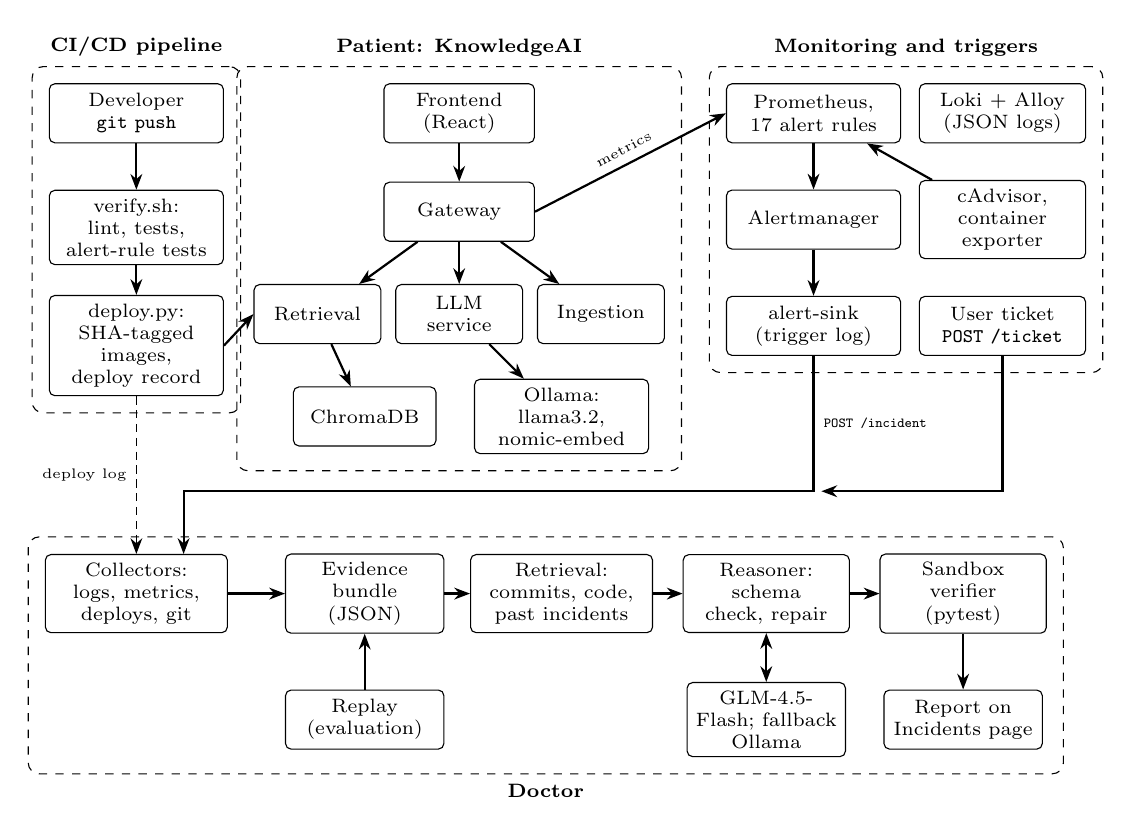
\begin{tikzpicture}[
  font=\scriptsize,
  box/.style={draw, rounded corners=2pt, align=center, fill=white, minimum height=0.75cm, inner sep=3pt, text width=#1},
  box/.default=2.0cm,
  grp/.style={draw, dashed, rounded corners=4pt, inner sep=6pt},
  arr/.style={-{Stealth[length=2mm]}, thick},
  dar/.style={-{Stealth[length=2mm]}, densely dashed}
]
% CI/CD
\node[box] (push) at (0,4.2) {Developer\\ \texttt{git push}};
\node[box] (ver) at (0,2.75) {verify.sh: lint, tests, alert-rule tests};
\node[box] (dep) at (0,1.25) {deploy.py: SHA-tagged images, deploy record};
% Patient
\node[box=1.7cm] (fe) at (4.1,4.2) {Frontend (React)};
\node[box=1.7cm] (gw) at (4.1,2.95) {Gateway};
\node[box=1.4cm] (ret) at (2.3,1.65) {Retrieval};
\node[box=1.4cm] (llm) at (4.1,1.65) {LLM service};
\node[box=1.4cm] (ing) at (5.9,1.65) {Ingestion};
\node[box=1.6cm] (chr) at (2.9,0.35) {ChromaDB};
\node[box=2.0cm] (oll) at (5.4,0.35) {Ollama: llama3.2, nomic-embed};
% Monitoring
\node[box=2.0cm] (prom) at (8.6,4.2) {Prometheus, 17 alert rules};
\node[box=2.0cm] (am) at (8.6,2.85) {Alertmanager};
\node[box=2.0cm] (sink) at (8.6,1.5) {alert-sink (trigger log)};
\node[box=1.9cm] (loki) at (11.0,4.2) {Loki + Alloy (JSON logs)};
\node[box=1.9cm] (cad) at (11.0,2.85) {cAdvisor, container exporter};
\node[box=1.9cm] (tick) at (11.0,1.5) {User ticket \texttt{POST /ticket}};
% Doctor
\node[box=2.1cm] (col) at (0,-1.9) {Collectors: logs, metrics, deploys, git};
\node[box=1.8cm] (bun) at (2.9,-1.9) {Evidence bundle (JSON)};
\node[box=2.1cm] (rnk) at (5.4,-1.9) {Retrieval: commits, code, past incidents};
\node[box=1.9cm] (rsn) at (8.0,-1.9) {Reasoner: schema check, repair};
\node[box=1.9cm] (vfy) at (10.5,-1.9) {Sandbox verifier (pytest)};
\node[box=1.8cm] (llmp) at (8.0,-3.5) {GLM-4.5-Flash; fallback Ollama};
\node[box=1.8cm] (rep) at (10.5,-3.5) {Report on Incidents page};
\node[box=1.8cm] (rpl) at (2.9,-3.5) {Replay (evaluation)};
\begin{scope}[on background layer]
\node[grp, fit=(push)(ver)(dep), label={[font=\scriptsize\bfseries]above:CI/CD pipeline}] {};
\node[grp, fit=(fe)(ret)(ing)(chr)(oll), label={[font=\scriptsize\bfseries]above:Patient: KnowledgeAI}] {};
\node[grp, fit=(prom)(sink)(loki)(tick), label={[font=\scriptsize\bfseries]above:Monitoring and triggers}] {};
\node[grp, fit=(col)(vfy)(llmp)(rep)(rpl), label={[font=\scriptsize\bfseries]below:Doctor}] {};
\end{scope}
\draw[arr] (push) -- (ver);
\draw[arr] (ver) -- (dep);
\draw[arr] (dep.east) -- (ret.west);
\draw[arr] (fe) -- (gw);
\draw[arr] (gw) -- (ret);
\draw[arr] (gw) -- (llm);
\draw[arr] (gw) -- (ing);
\draw[arr] (ret) -- (chr);
\draw[arr] (llm) -- (oll);
\draw[arr] (gw.east) -- node[above, sloped, font=\tiny]{metrics} (prom.west);
\draw[arr] (prom) -- (am);
\draw[arr] (am) -- (sink);
\draw[arr] (sink.south) -- node[right, font=\tiny]{\texttt{POST /incident}} (8.6,-0.6) -| ([xshift=6mm]col.north);
\draw[arr] (tick.south) |- (8.7,-0.6);
\draw[arr] (cad) -- (prom);
\draw[arr] (col) -- (bun);
\draw[arr] (bun) -- (rnk);
\draw[arr] (rnk) -- (rsn);
\draw[arr] (rsn) -- (vfy);
\draw[{Stealth[length=2mm]}-{Stealth[length=2mm]}, thick] (rsn) -- (llmp);
\draw[arr] (vfy) -- (rep);
\draw[arr] (rpl) -- (bun);
\draw[dar] (dep.south) -- node[left, font=\tiny]{deploy log} (col.north);
\end{tikzpicture}
\caption{Architecture of the system. Dashed boxes group the four subsystems. Solid arrows are requests or data flow (the arrow from deploy.py is the deploy of the patient), and the dashed arrow is the deploy log that the doctor reads. The pipeline ends at the deploy record, and only an alert, a ticket or a replay starts a diagnosis.}
\label{fig:arch}
\end{figure}

\subsection{Triggers and Evidence Windows}
Alerts on the same service within ten minutes are joined into one incident, because one fault often fires several rules. For a ticket, the doctor finds the onset from the symptom metrics around the time the user gave, and uses that as $t_a$. The doctor then waits until the incident window has closed. The two windows are defined in Eq.~\eqref{eq:windows}:
\begin{equation}
W_{\mathrm{inc}}=[t_a-\Delta_b,\; t_a+\Delta_a],\qquad W_{\mathrm{base}}=[t_a-\Delta_b-\Delta_0,\; t_a-\Delta_b],
\label{eq:windows}
\end{equation}
where $\Delta_b=600$~s and $\Delta_a=60$~s set the incident window and $\Delta_0=1800$~s is the length of the baseline. Ten minutes before the alert is enough for the slowest rule, the memory rule, which waits three minutes. A 30-minute baseline has enough background traffic that a few slow requests do not change its average.

\subsection{Evidence Bundle}
The collectors fetch the warning and error lines from Loki for both windows, group them by log signature, and mark the groups that are new in the incident window. From Prometheus they fetch traffic, latency, error, memory, restart and service-status series. A series is counted as a notable change, and added to the set $\mathcal{N}$, when Eq.~\eqref{eq:notable} holds:
\begin{equation}
\max_{W_{\mathrm{inc}}} m \;>\; \max\!\bigl(\rho\,\bar{m}_{W_{\mathrm{base}}},\; \bar{m}_{W_{\mathrm{base}}}+\epsilon\bigr),
\label{eq:notable}
\end{equation}
with $\rho=1.5$ and $\epsilon=10^{-6}$. The bundle also holds the deploy records from the six hours before $t_a$, every patient commit that those deploys shipped with its diff, the knowledge-base loads, and the source lines around each stack-trace frame. Commits that only change experimenter files (fault scripts, recorded incidents and the doctor itself) are dropped, because their diffs would give away the injected fault. The bundle is saved to disk before any reasoning starts, so every diagnosis can be replayed later.

\subsection{Commit Ranking}
The time filter alone gave 22 to 46 candidate commits per push incident, too many diffs for a 6,500-token prompt, so the doctor ranks them. The lexical part takes terms from the evidence with the weights in Eq.~\eqref{eq:weights}:
\begin{equation}
w_E(t)=\sum_{g\in\mathcal{L}}\Bigl(\omega_g\,n^{\mathrm{msg}}_g(t)+2\omega_g\,n^{\mathrm{file}}_g(t)+n^{\mathrm{stack}}_g(t)\Bigr)+n_a(t)+\sum_{m\in\mathcal{N}}\Bigl(2\,\mathbf{1}[t\in V_m]+n_m(t)\Bigr),
\label{eq:weights}
\end{equation}
where $\omega_g=3$ for a log group that was not in the baseline and $1$ otherwise. Here $n^{\mathrm{msg}}_g$, $n^{\mathrm{file}}_g$ and $n^{\mathrm{stack}}_g$ count term $t$ in the message, the error file path and the stack lines of group $g$, $n_a$ counts it in the alert labels, and $V_m$ is a short list of symptom words for metric $m$. For example, a rising fallback counter adds ``embed'', ``fallback'' and ``timeout''. This list is written once for all incidents and has no knowledge of any injected fault. The lexical score of a commit $c$ is
\begin{equation}
s_{\mathrm{lex}}(c)=\frac{\sum_{t\in T_E\cap T_c} w_E(t)\,\min\bigl(n_c(t),3\bigr)}{\sqrt{\max(1,|T_c|)}},
\label{eq:lex}
\end{equation}
where $T_E$ is the set of evidence terms. Dividing by the square root of the commit's term count stops a large commit from winning just because it touches many identifiers. With this change and with the doctor's own commits excluded, the guilty commit of the first timeout incident moved from 11th of 45 to first of 26. The semantic score in Eq.~\eqref{eq:sem} is the highest cosine similarity between an evidence summary $q$ (the alert, the top log groups and the notable changes) and the diff $d_{c,f}$ of each file $f$ in the commit:
\begin{equation}
s_{\mathrm{sem}}(c)=\max_{f\in F_c}\cos\bigl(\phi(q),\phi(d_{c,f})\bigr).
\label{eq:sem}
\end{equation}
The final score combines the two parts:
\begin{equation}
S(c)=\alpha\,\frac{s_{\mathrm{lex}}(c)}{\max_{c'}s_{\mathrm{lex}}(c')}+(1-\alpha)\,s_{\mathrm{sem}}(c),\qquad \alpha=0.6.
\label{eq:score}
\end{equation}
The top five commits by $S(c)$ are the only SHAs that the model is allowed to name. We give the lexical part more weight because identifiers from a stack trace are exact evidence, while the embedding of a diff mostly captures its topic. The same embeddings fetch up to four code chunks at the running commit and up to three earlier incidents.

\subsection{Prompt and Evidence Arms}
Every model gets the same system prompt. It defines the five classes and tells the model to first decide whether demand went up or capacity went down, by comparing the traffic in the two windows. It also says that a deploy existing is not evidence by itself. The sections included in the user prompt define three evidence arms. \emph{logs\_only} has the alert, related alerts, notable changes, metrics, log groups and the source at stack-trace lines. \emph{logs\_commits} adds the deploy records, knowledge-base loads, ranked commits with their diffs and the code chunks. \emph{logs\_commits\_incidents} also adds similar past incidents with how they were resolved. If the prompt is longer than 6,500 tokens, the longest optional section is cut by 30\% until it fits. This way a model with an 8k context sees the same evidence as a model with a much larger one.

\subsection{Schema-Checked Reasoning}
The model must answer with a JSON object holding the class, a demand-versus-capacity verdict, one to three hypotheses and a fix. For Ollama, the JSON schema is passed as the output format. GLM is asked for a JSON object shaped like an example, because the Z.ai endpoint ignored the schema in our tests. The doctor checks the answer against the schema and against rules that a schema cannot express. A named SHA must be one of the candidates, a capacity incident cannot blame a commit, and a code fix must contain edits. If the check fails, the model gets one more turn with the list of errors.

Fixes are asked for as search-and-replace edits and not as unified diffs, because small models rarely write a diff that \texttt{git apply} accepts. The doctor turns the edits into a diff against the running commit itself. When a model copies the guilty diff in the wrong direction, the doctor applies the edit in reverse and records that it did so.

\subsection{Sandbox Verification}
The verifier exports the repository at the running SHA with \texttt{git archive}, applies the diff, and runs the patient's test suite in a subprocess with a 420-second limit. A fix is marked \emph{verified} only if the diff applies and every test passes. In the evaluation, the fault's acceptance test also runs on the copy and is reported separately: the suite shows that nothing else broke, the acceptance test that the fault is fixed. A restart or other action cannot be tested on a copy, so it stays \emph{unverified}. Algorithm~\ref{alg:diagnose} gives the full diagnosis step, and Fig.~\ref{fig:workflow} shows the flow from the trigger to the report.

\begin{algorithm}[!t]
\caption{Diagnose one incident}
\label{alg:diagnose}
\SetKwInOut{Input}{Input}\SetKwInOut{Output}{Output}
\Input{bundle $B$, evidence arm $r$, providers $P$, acceptance tests $A$}
\Output{report with diagnosis $y$, retrieval results and verification status}
\eIf{$r=$ logs\_only}{$R\leftarrow\emptyset$; $\mathit{code}\leftarrow\emptyset$\;}{
  $R\leftarrow$ top 5 of $\mathcal{C}$ by $S(c)$ (Eq.~\ref{eq:score})\;
  $\mathit{code}\leftarrow$ chunks near stack-trace files and the top 2 commits' files\;}
$I\leftarrow$ up to 3 earlier incidents if $r=$ logs\_commits\_incidents, else $\emptyset$\;
$\pi\leftarrow$ \textsc{BuildPrompt}$(B,r,R,\mathit{code},I)$, trimmed to 6,500 tokens\;
\ForEach{provider $p\in P$}{
  $o\leftarrow p(\pi)$; $E\leftarrow$ schema and rule errors of $o$\;
  \lIf{$E\neq\emptyset$}{$o\leftarrow p(\pi\,\|\,\textsc{Repair}(o,E))$}
  \lIf{$o$ is schema-valid}{\textbf{break}}
}
\lIf{no provider returned a valid $o$}{\Return status \emph{failed}}
$y\leftarrow$ \textsc{Normalise}$(o,R)$: resolve SHAs, clamp confidences, sort hypotheses, log violations\;
\uIf{$y.\mathit{fix}$ is a code or config change}{
  $\delta\leftarrow$ \textsc{EditsToDiff}$(y.\mathit{fix}.\mathit{edits}, B.\mathit{live\_sha})$\;
  copy repository at $B.\mathit{live\_sha}$; apply $\delta$; run test suite and $A$\;
  status $\leftarrow$ \emph{verified} if $\delta$ applied and the suite passed, else \emph{unverified}\;}
\lElse{status $\leftarrow$ \emph{unverified, needs human review}}
\Return report$(y, R, I, \text{status})$\;
\end{algorithm}

\begin{figure}[!t]
\centering
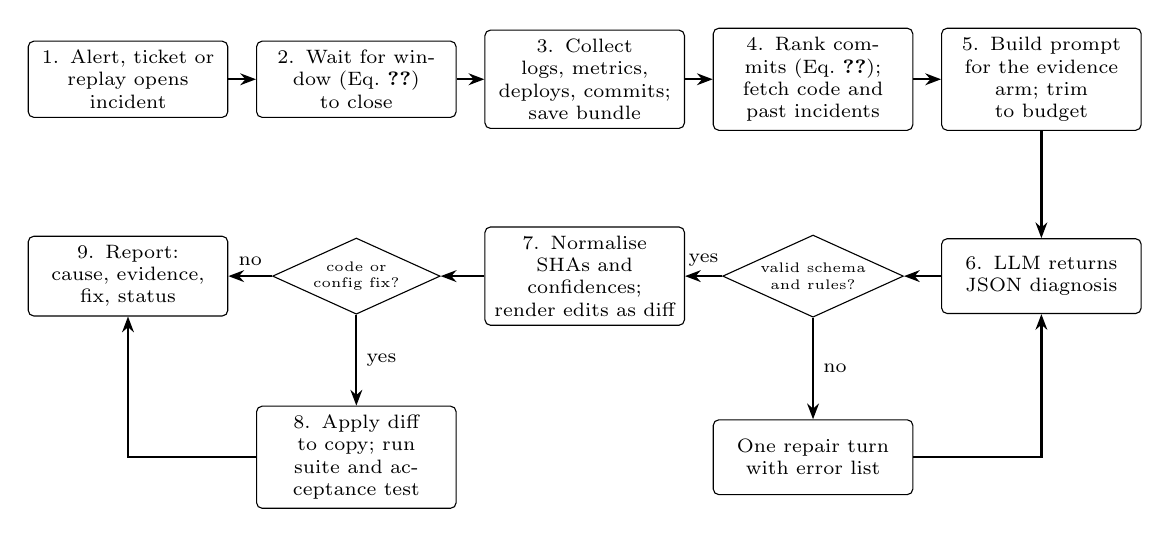
\begin{tikzpicture}[
  font=\scriptsize,
  st/.style={draw, rounded corners=2pt, align=center, text width=2.3cm, minimum height=0.95cm, fill=white},
  dec/.style={draw, diamond, aspect=2.2, align=center, inner sep=1pt, font=\tiny},
  arr/.style={-{Stealth[length=2mm]}, thick}
]
\node[st] (s1) at (0,0) {1. Alert, ticket or replay opens incident};
\node[st] (s2) at (2.9,0) {2. Wait for window (Eq.~\ref{eq:windows}) to close};
\node[st] (s3) at (5.8,0) {3. Collect logs, metrics, deploys, commits; save bundle};
\node[st] (s4) at (8.7,0) {4. Rank commits (Eq.~\ref{eq:score}); fetch code and past incidents};
\node[st] (s5) at (11.6,0) {5. Build prompt for the evidence arm; trim to budget};
\node[st] (s6) at (11.6,-2.5) {6. LLM returns JSON diagnosis};
\node[dec] (d1) at (8.7,-2.5) {valid schema\\and rules?};
\node[st] (s7) at (5.8,-2.5) {7. Normalise SHAs and confidences; render edits as diff};
\node[dec] (d2) at (2.9,-2.5) {code or\\config fix?};
\node[st] (s8) at (2.9,-4.8) {8. Apply diff to copy; run suite and acceptance test};
\node[st] (s9) at (0,-2.5) {9. Report: cause, evidence, fix, status};
\node[st] (rep) at (8.7,-4.8) {One repair turn with error list};
\draw[arr] (s1) -- (s2);
\draw[arr] (s2) -- (s3);
\draw[arr] (s3) -- (s4);
\draw[arr] (s4) -- (s5);
\draw[arr] (s5) -- (s6);
\draw[arr] (s6) -- (d1);
\draw[arr] (d1) -- node[above]{yes} (s7);
\draw[arr] (d1) -- node[right]{no} (rep);
\draw[arr] (rep.east) -| (s6.south);
\draw[arr] (s7) -- (d2);
\draw[arr] (d2) -- node[right]{yes} (s8);
\draw[arr] (d2) -- node[above]{no} (s9);
\draw[arr] (s8.west) -| (s9.south);
\end{tikzpicture}
\caption{Workflow of one diagnosis, from the trigger to the report. The failure path after a second invalid answer, which ends the diagnosis as \emph{failed}, is left out to keep the figure simple.}
\label{fig:workflow}
\end{figure}

% ======================================================================
\section{Experimental Setup}\label{sec:setup}

\subsection{Test Environment}
The replays and the Llama live runs were done on one laptop with Windows~11, an NVIDIA RTX~5070 with 8~GB, 15~GB of RAM, Docker Desktop and a local Ollama server. The four FastAPI services of the patient run in Python~3.10 images with FastAPI~0.141, ChromaDB~1.5.9 and httpx~0.28. Monitoring uses Prometheus~3.5.0, Alertmanager~0.28.1, Loki~3.5.3, Grafana Alloy~1.10.2 and cAdvisor~0.53.0. The patient's test suite has 137 test functions, and the linter is Ruff~0.15. Every deploy went through a local bare git repository whose post-receive hook runs the same \texttt{verify.sh} and \texttt{deploy.sh} scripts as the GitHub Actions workflow.

\subsection{Faults and Dataset}
Table~\ref{tab:faults} lists the eight faults. Push faults are real commits with ordinary messages, placed among harmless distractor commits. In run~1, a distractor ships after the guilty commit in the same deploy. In run~2, the guilty commit ships in an earlier deploy, and a deploy with only distractors follows it. Each push fault passes the existing tests and the linter, so it would really ship, but it fails its own acceptance test.

Background traffic of 0.2 chats and 0.4 searches per second ran during the whole campaign, with ten-minute breaks between runs. Each fault was run twice, which gave 16 incidents: 8 push, 6 environment and 2 data. We discarded eight more runs for recorded reasons, among them two faults whose first settings did not reproduce.

\begin{table}[!t]
\caption{Injected Faults}
\label{tab:faults}
\centering
\small
\begin{tabularx}{\textwidth}{L{2.6cm}L{1.9cm}L{3.1cm}Y}
\toprule
\textbf{Fault} & \textbf{Delivery} & \textbf{True class} & \textbf{What happens} \\
\midrule
f1 embed timeout & push & code\_defect & Embedding timeout cut from 45~s to 10~s; when Ollama is busy, a silent fallback returns meaningless vectors \\
f2 capacity & environment & capacity & A chat surge saturates the single local model; no commit is guilty \\
f3 retrieval down & environment & dependency\_failure & Retrieval container stopped \\
f3b bad address & environment & dependency\_failure & Gateway pointed at a host that does not exist \\
f4 memory leak & push & code\_defect & Retrieval cache never evicts; memory climbs until the container is killed \\
f5 typo & push & code\_defect & Attribute typo on the branch taken only by keyword queries \\
f6 tight timeout & push & code\_defect & Retrieval call timeout set to 0.05~s, so about 7\% of chats fail \\
f7 missing docs & data & data\_issue & A knowledge-base version with 6 of 10 documents missing is loaded \\
\bottomrule
\end{tabularx}
\end{table}

\subsection{Baselines}
The first baseline blames the most recent deploy. It names the newest in-scope commit of that deploy and calls the incident a code defect, which is what an engineer usually does when a page comes right after a release. The second baseline is the logs\_only arm: what the model can work out from telemetry alone.

\subsection{Metrics}
A hypothesis matches the truth if it names the guilty commit. When no commit is guilty, it matches if it names no commit and names an acceptable component. We report the following metrics:
\begin{itemize}
\item \emph{acc@$k$}: the share of incidents with a matching hypothesis in the top $k$, the usual ranking measure;
\item \emph{false attribution}: the share of no-commit incidents where the top hypothesis names a commit, since this is the mistake that sends an engineer to revert innocent code;
\item \emph{class accuracy}: the share of incidents with the right class, because the class decides what to do (revert, restart or scale);
\item \emph{fix verified (suite)} and \emph{fix correct (acceptance)}: the shares of push incidents whose fix passes the suite and the fault's acceptance test, because a fix that does not work is of no use;
\item \emph{seconds} and \emph{tokens} per diagnosis, to show the cost.
\end{itemize}
Eq.~\eqref{eq:metrics} defines the two accuracy measures for a set of incidents $I$ and its no-commit subset $I_0$:
\begin{equation}
\mathrm{acc@}k=\frac{1}{|I|}\sum_{i\in I}\mathbf{1}\bigl[\exists j\le k:\ \mathrm{match}(h^{(i)}_j)\bigr],\qquad
\mathrm{FA}=\frac{1}{|I_0|}\sum_{i\in I_0}\mathbf{1}\bigl[h^{(i)}_1\ \text{names a commit}\bigr].
\label{eq:metrics}
\end{equation}
Each configuration ran three times, with seeds 1000, 1001 and 1002, and we report the mean $\pm$ sample standard deviation of each metric over the three repeats.

\subsection{Live Test of the Chosen Setup}
Full evidence gave GLM its highest acc@1 over all faults (0.46, against 0.38 with commits and 0.25 with logs only), so we tested this setup live with Claude Opus 5.5 (\texttt{claude-}\allowbreak\texttt{opus-5-5})~\cite{anthropic2026opus55}, using the same campaign script and eight faults, each run twice. The runs took place on 22 and 24 November 2026 on a Google Cloud VM (g2-standard-8, one NVIDIA L4 GPU) that hosted the patient and its Ollama models. The doctor called Claude through Anthropic's API with the replay budgets and effort set to high; Opus 5.5 always reasons internally, so no temperature was sent. The first two f7 attempts crashed on a missing file and were re-run with the same partial knowledge base (version 405bbf0b9802) as the Llama f7 runs. We compare these runs with the September live runs of Llama~3.2 on the laptop, using the replays' scoring function.

\subsection{Parameters}
Table~\ref{tab:params} lists every setting we used. GLM-4.5-Flash~\cite{glm2025glm45} ran on Z.ai's free tier with thinking turned off, because with it on, the model used the whole 2,500-token answer allowance before writing any JSON. The local models, Llama~3 8B and Llama~3.2 3B~\cite{grattafiori2024llama3}, ran through Ollama's native chat API.

\begin{table}[!t]
\caption{Parameters Used in All Experiments}
\label{tab:params}
\centering
\small
\begin{tabular}{lll}
\toprule
\textbf{Group} & \textbf{Parameter} & \textbf{Value} \\
\midrule
Windows & $\Delta_b$, $\Delta_a$, $\Delta_0$ & 600 s, 60 s, 1800 s \\
 & Deploy look-back & 6 h \\
 & Alert grouping & same service within 10 min \\
Evidence & Notable-change ratio $\rho$, $\epsilon$ & 1.5, $10^{-6}$ \\
 & Log groups in prompt & 15 \\
Retrieval & $\alpha$ (lexical weight) & 0.6 \\
 & Term count cap & 3 \\
 & Candidate commits shown & top 5 \\
 & Code chunks / past incidents & 4 / 3 \\
 & Embedding model & nomic-embed-text \\
Reasoning & Prompt budget / answer budget & 6,500 / 2,500 tokens \\
 & Ollama context (replay) & 16,384 tokens \\
 & Repair turns / call cap per run & 1 / 6 \\
 & GLM thinking mode & disabled \\
Verification & Suite / acceptance timeout & 420 s / 180 s \\
Evaluation & Repeats and seeds & 3; 1000, 1001, 1002 \\
 & Arms & logs\_only, logs\_commits, logs\_commits\_incidents \\
 & Models & GLM-4.5-Flash, Llama~3 8B, Llama~3.2 3B \\
Campaign & Background traffic & 0.2 chat/s, 0.4 search/s \\
 & Runs per fault, cool-down & 2, 10 min \\
Live (Llama) & Model, context, prompt / answer & Llama~3.2, 4,096, 3,000 / 900 tokens \\
Live (Claude) & Model, prompt / answer, effort & Opus 5.5, 6,500 / 2,500 tokens, high \\
\bottomrule
\end{tabular}
\end{table}

% ======================================================================
\section{Results and Analysis}\label{sec:results}

The evaluation scored 336 different replays: 144 for GLM (three arms, 16 incidents and three repeats), 144 for Llama~3, and 48 for Llama~3.2 with full evidence. GLM gave a valid answer in 141 of its 144 replays, and the local models gave one in all of theirs.

\subsection{RQ1: Root-Cause Accuracy and False Attribution}
Table~\ref{tab:main} compares the three models with full evidence against the most-recent-deploy baseline. The baseline is wrong on every environment fault, because there is always a deploy in the window. It also never names the guilty commit of a push fault, because in every push run a distractor commit shipped after it. If we only ask whether the guilty commit was inside the latest deploy, the baseline scores 0.50. GLM found the right cause in 0.56 of environment faults, and in 0.89 within its top three, over three times Llama~3's 0.17. It also blamed an innocent commit in only 0.11 of them, against 0.67 for Llama~3. On push faults GLM reached 0.38 acc@1 and Llama~3 reached 0.33, while Llama~3.2 almost never named the guilty commit. GLM also had the best class accuracy, at 0.81.

\begin{table}[!t]
\caption{Full-Evidence Results Against the Baseline (mean $\pm$ std over 3 repeats; best in bold)}
\label{tab:main}
\centering
\setlength{\tabcolsep}{4pt}
\resizebox{\textwidth}{!}{%
\begin{tabular}{lcccccccc}
\toprule
 & \multicolumn{3}{c}{\textbf{Environment (6 incidents)}} & \multicolumn{3}{c}{\textbf{Push (8 incidents)}} & \textbf{All (16)} & \\
\cmidrule(lr){2-4}\cmidrule(lr){5-7}\cmidrule(lr){8-8}
\textbf{Configuration} & acc@1 & acc@3 & FA $\downarrow$ & acc@1 & suite & accept. & class & s / tokens \\
\midrule
Most recent deploy & 0.00 & 0.00 & 1.00 & 0.00 & 0.00 & 0.00 & 0.50 & -- / 0 \\
GLM-4.5-Flash & \textbf{0.56}$\pm$0.10 & \textbf{0.89}$\pm$0.10 & \textbf{0.11}$\pm$0.10 & \textbf{0.38}$\pm$0.00 & \textbf{0.75}$\pm$0.00 & \textbf{0.71}$\pm$0.07 & \textbf{0.81}$\pm$0.00 & 54.7 / 14.2k \\
Llama 3 8B & 0.17$\pm$0.17 & 0.17$\pm$0.17 & 0.67$\pm$0.17 & 0.33$\pm$0.07 & 0.33$\pm$0.07 & 0.29$\pm$0.07 & 0.69$\pm$0.06 & 11.1 / 11.0k \\
Llama 3.2 3B & 0.28$\pm$0.10 & 0.44$\pm$0.19 & 0.22$\pm$0.10 & 0.04$\pm$0.07 & 0.08$\pm$0.07 & 0.08$\pm$0.07 & 0.58$\pm$0.10 & 5.5 / 10.6k \\
\bottomrule
\end{tabular}}
\end{table}

Fig.~\ref{fig:ablation} and Table~\ref{tab:ablation} show the ablation, where one part of the evidence is added at a time. For Llama~3, adding commits raised push-fault acc@1 from 0.00 to 0.21, and adding past incidents raised it to 0.33. On environment faults, the same commits raised false attribution from 0.00 to 0.83 and dropped acc@1 from 0.39 to 0.00. Past incidents only brought false attribution back down to 0.67. In other words, when the 8B model sees a list of commits it picks one, even though the prompt says that a deploy is not evidence by itself.

GLM got the push-fault gain without most of this harm. Its false attribution rose only to 0.17 with commits and fell to 0.11 with past incidents. Past incidents also raised GLM's class accuracy on environment faults from 0.33 to 0.83, because a resolved ``retrieval container stopped'' incident shows it what a dependency failure looks like.

\begin{figure}[!t]
\centering
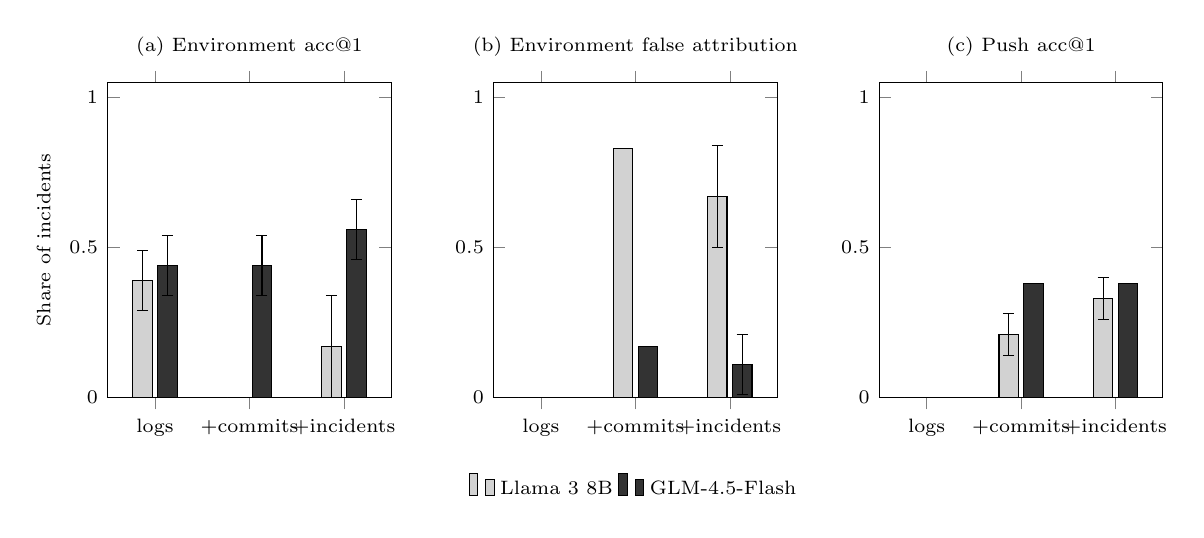
\begin{tikzpicture}
\begin{groupplot}[
  group style={group size=3 by 1, horizontal sep=1.3cm},
  scale only axis, width=3.6cm, height=4.0cm,
  ybar, /pgf/bar width=7pt, ymin=0, ymax=1.05,
  symbolic x coords={L,LC,LCI}, xtick=data,
  xticklabels={logs, +commits, +incidents},
  xticklabel style={font=\scriptsize},
  yticklabel style={font=\scriptsize},
  ylabel style={font=\scriptsize},
  title style={font=\scriptsize},
  enlarge x limits=0.25,
  error bars/y dir=both, error bars/y explicit,
  legend style={font=\scriptsize, at={(0.5,-0.22)}, anchor=north, legend columns=2, draw=none},
]
\nextgroupplot[title={(a) Environment acc@1}, ylabel={Share of incidents}]
\addplot[fill=gray!35, draw=black] coordinates {(L,0.39) +- (0,0.10) (LC,0.00) +- (0,0.00) (LCI,0.17) +- (0,0.17)};
\addplot[fill=black!80, draw=black] coordinates {(L,0.44) +- (0,0.10) (LC,0.44) +- (0,0.10) (LCI,0.56) +- (0,0.10)};
\nextgroupplot[title={(b) Environment false attribution}]
\addplot[fill=gray!35, draw=black] coordinates {(L,0.00) +- (0,0.00) (LC,0.83) +- (0,0.00) (LCI,0.67) +- (0,0.17)};
\addplot[fill=black!80, draw=black] coordinates {(L,0.00) +- (0,0.00) (LC,0.17) +- (0,0.00) (LCI,0.11) +- (0,0.10)};
\legend{Llama 3 8B, GLM-4.5-Flash}
\nextgroupplot[title={(c) Push acc@1}]
\addplot[fill=gray!35, draw=black] coordinates {(L,0.00) +- (0,0.00) (LC,0.21) +- (0,0.07) (LCI,0.33) +- (0,0.07)};
\addplot[fill=black!80, draw=black] coordinates {(L,0.00) +- (0,0.00) (LC,0.38) +- (0,0.00) (LCI,0.38) +- (0,0.00)};
\end{groupplot}
\end{tikzpicture}
\caption{Evidence ablation for Llama~3 8B and GLM-4.5-Flash. The bars are means over three seeded repeats and the error bars are $\pm$ one standard deviation. Lower is better in panel (b).}
\label{fig:ablation}
\end{figure}

\begin{table}[!t]
\caption{Ablation: Effect of Each Evidence Component (mean $\pm$ std over 3 repeats)}
\label{tab:ablation}
\centering
\footnotesize
\setlength{\tabcolsep}{5pt}
\begin{tabular}{llccccc}
\toprule
\textbf{Model} & \textbf{Arm} & Env acc@1 & Env FA $\downarrow$ & Push acc@1 & Push accept. & Class (all) \\
\midrule
Llama 3 8B & logs only & \textbf{0.39}$\pm$0.10 & \textbf{0.00}$\pm$0.00 & 0.00$\pm$0.00 & 0.25$\pm$0.00 & 0.65$\pm$0.07 \\
 & + commits & 0.00$\pm$0.00 & 0.83$\pm$0.00 & 0.21$\pm$0.07 & 0.25$\pm$0.00 & 0.54$\pm$0.04 \\
 & + past incidents & 0.17$\pm$0.17 & 0.67$\pm$0.17 & \textbf{0.33}$\pm$0.07 & \textbf{0.29}$\pm$0.07 & \textbf{0.69}$\pm$0.06 \\
\midrule
GLM-4.5-Flash & logs only & 0.44$\pm$0.10 & \textbf{0.00}$\pm$0.00 & 0.00$\pm$0.00 & 0.25$\pm$0.00 & 0.52$\pm$0.07 \\
 & + commits & 0.44$\pm$0.10 & 0.17$\pm$0.00 & \textbf{0.38}$\pm$0.00 & \textbf{0.71}$\pm$0.07 & 0.62$\pm$0.00 \\
 & + past incidents & \textbf{0.56}$\pm$0.10 & 0.11$\pm$0.10 & \textbf{0.38}$\pm$0.00 & \textbf{0.71}$\pm$0.07 & \textbf{0.81}$\pm$0.00 \\
\bottomrule
\end{tabular}
\end{table}

Retrieval puts a limit on push-fault accuracy. Fig.~\ref{fig:rank} shows the rank of the guilty commit after re-ranking, next to the size of the time-filtered set. The time filter always contained the guilty commit, and re-ranking put it in the top five for 5 of the 8 incidents, so no model could score above 0.62 acc@1 on this set. GLM named it in all three repeats for three of those five (f1 in both runs and f6 run~1). The two memory-leak incidents ranked 7th and 11th. Their diff adds a cache, which reads like an optimisation and not like the memory growth that fills the evidence. The f1 run~1 ranking was used while we fixed the length division in Eq.~\eqref{eq:lex}, so that one incident is not held out.

\begin{figure}[!t]
\centering
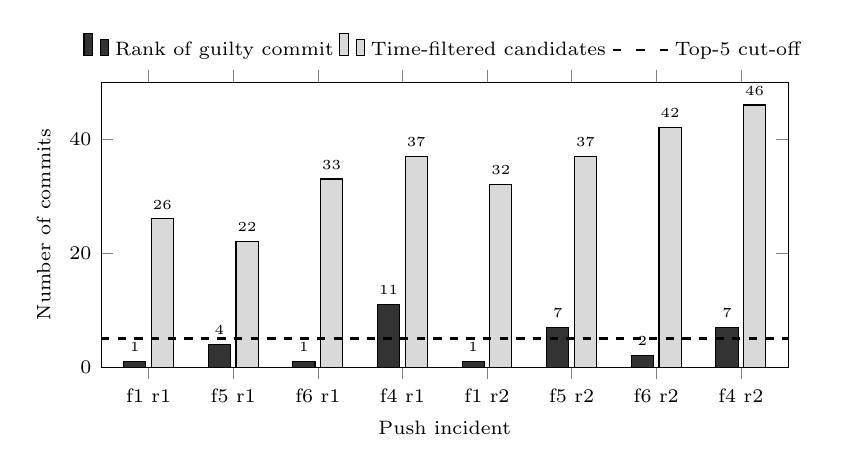
\begin{tikzpicture}
\begin{axis}[
  width=0.85\textwidth, height=5.2cm,
  ybar, bar width=8pt, ymin=0, ymax=50,
  symbolic x coords={a,b,c,d,e,f,g,h}, xtick=data,
  xticklabels={f1 r1,f5 r1,f6 r1,f4 r1,f1 r2,f5 r2,f6 r2,f4 r2},
  xticklabel style={font=\scriptsize}, yticklabel style={font=\scriptsize},
  ylabel={Number of commits}, ylabel style={font=\scriptsize},
  xlabel={Push incident}, xlabel style={font=\scriptsize},
  legend style={font=\scriptsize, at={(0.5,1.04)}, anchor=south, legend columns=3, draw=none},
  nodes near coords, nodes near coords style={font=\tiny},
  enlarge x limits=0.08,
]
\addplot[fill=black!80, draw=black] coordinates {(a,1) (b,4) (c,1) (d,11) (e,1) (f,7) (g,2) (h,7)};
\addplot[fill=gray!30, draw=black] coordinates {(a,26) (b,22) (c,33) (d,37) (e,32) (f,37) (g,42) (h,46)};
\draw[dashed, thick] (rel axis cs:0,0.1) -- (rel axis cs:1,0.1);
\addlegendimage{dashed, thick, line legend}
\legend{Rank of guilty commit, Time-filtered candidates, Top-5 cut-off}
\end{axis}
\end{tikzpicture}
\caption{Rank of the guilty commit after hybrid re-ranking (dark bars) and the number of candidates in the six-hour time filter (light bars) for the eight push incidents. Ranks above the dashed line at 5 never reach the prompt.}
\label{fig:rank}
\end{figure}

\subsection{RQ2: Fix Verification}
The suite and acceptance columns of Table~\ref{tab:main} answer RQ2. GLM's fixes passed the full test suite in 0.75 of push incidents and the fault's acceptance test in 0.71, against 0.33 and 0.29 for Llama~3 and 0.08 for Llama~3.2. None of GLM's 72 push-fault replays needed the reversed-edit correction, so its acceptance rate is entirely its own work. Llama~3 needed it in 3 of its 96 push replays; without it, its logs\_commits acceptance would fall from 0.25 to 0.17.

The fix is judged by the file it repairs, so f5's typo fix passed its acceptance test in every GLM repeat even though GLM did not name f5's guilty commit. The stack trace of f5 points at the broken line, and the two f5 incidents give logs\_only all of its 0.25 acceptance.

\subsection{Data Fault and Live Behaviour}
In the replays, no model understood the data fault. GLM scored 0.50 acc@1 on f7 only because the scorer gives credit for the right component when no commit is guilty. Its explanations named a ChromaDB connection problem, and its class was right in 0 of 18 replays over the three arms. Monitoring also missed f7 in both Llama runs: refusals rose to about 20\%, under the 30\% alert threshold, so a user ticket woke the doctor, and the reports came 29 and 32~s later.

Fig.~\ref{fig:live} shows the live timings for the 14 incidents that raised an alert, with the live doctor running Llama~3.2 at a 4k context. Environment faults raised an alert after a median of 78~s and push faults after 323~s, which includes verify, build and deploy and the minutes of growth that the memory rule needs. From alert to report the doctor took a median of 105~s for push faults and 120~s for environment faults, which includes the 60-second wait for the incident window to close. The live doctor got the class right in only 4 of 16 runs and answered ``capacity'' in 12 of them. The same bundles replayed with GLM reach 0.81 class accuracy, so the weak live results come from the small model and the shared GPU, not from the evidence.

Table~\ref{tab:live} tests this claim live. Each fault ran once per round, so the table gives counts, and the replays remain the source of the seeded, repeated results. With full evidence, Claude Opus 5.5 got the class right in 15 of 16 runs and the cause in 14 of 16, against 4 and 5 for Llama~3.2, including all six environment runs and 6 of 8 push runs (Llama~3.2: 2 of 6 and 1 of 8). Neither model blamed a commit for a non-push fault. Claude's fixes passed the test suite in 6 of 8 push runs, and Llama~3.2's in none. The median time from alert or ticket to report was 105~s against 103~s, and the 16 Claude diagnoses cost USD 2.13.

Llama~3.2's 2 of 2 on the data fault comes from the scorer's component credit; its class was wrong in both runs (capacity and code\_defect). Claude classed both f7 runs as data\_issue, named the missing document topics (library, scholarships and placements), and in round 2 named the partial knowledge-base version 405bbf0b9802. Its reports came 26~s and 27~s after the user ticket. Claude missed only f1, the silent-fallback fault, in both runs (round 1 classed data\_issue, round 2 code\_defect with the wrong cause); monitoring raised no alert for f1, so a ticket woke the doctor. Monitoring missed 4 runs in Claude's campaign (f1 and f7, twice each) and 2 in Llama's (f7 twice). With the same kind of evidence, the strong model diagnosed almost every fault, which supports the replay result.

\begin{table}[!t]
\caption{Live Runs: Llama 3.2 3B vs Claude Opus 5.5 (counts over 16 runs)}
\label{tab:live}
\centering
\small
\begin{tabular}{lcc}
\toprule
 & \textbf{Llama 3.2 3B} & \textbf{Claude Opus 5.5} \\
 & (laptop, Sept.) & (cloud VM, Nov.) \\
\midrule
Runs & 16 & 16 \\
Class correct & 4/16 & \textbf{15/16} \\
acc@1 & 5/16 & \textbf{14/16} \\
\quad environment / data / push & 2/6, 2/2, 1/8 & 6/6, 2/2, 6/8 \\
acc@3 & 5/16 & \textbf{14/16} \\
False attribution, non-push $\downarrow$ & 0/8 & 0/8 \\
Fix verified, test suite (push) & 0/8 & \textbf{6/8} \\
Median alert/ticket to report (s) & 103 & 105 \\
Median evidence in the prompt (tokens) & 2,985 & 6,229 \\
Doctor API cost for 16 runs (USD) & 0 & 2.13 \\
\bottomrule
\end{tabular}
\end{table}

\begin{figure}[!t]
\centering
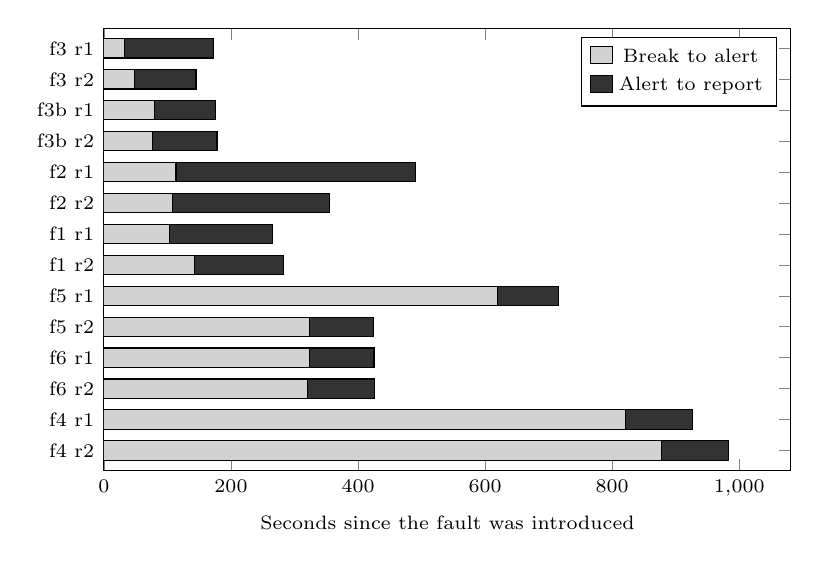
\begin{tikzpicture}
\begin{axis}[
  width=0.85\textwidth, height=7.2cm,
  xbar stacked, bar width=7pt, xmin=0,
  symbolic y coords={a,b,c,d,e,f,g,h,i,j,k,l,m,n},
  ytick=data, yticklabels={f3 r1,f3 r2,f3b r1,f3b r2,f2 r1,f2 r2,f1 r1,f1 r2,f5 r1,f5 r2,f6 r1,f6 r2,f4 r1,f4 r2}, y dir=reverse,
  yticklabel style={font=\scriptsize}, xticklabel style={font=\scriptsize},
  xlabel={Seconds since the fault was introduced}, xlabel style={font=\scriptsize},
  legend style={font=\scriptsize, at={(0.98,0.98)}, anchor=north east},
  enlarge y limits=0.05,
]
\addplot[fill=gray!35, draw=black] coordinates {(33.0,a) (47.9,b) (79.0,c) (77.0,d) (113.5,e) (108.5,f) (103.6,g) (142.6,h) (620.0,i) (323.0,j) (323.0,k) (321.0,l) (821.2,m) (877.2,n)};
\addplot[fill=black!80, draw=black] coordinates {(139.0,a) (97.1,b) (96.0,c) (101.0,d) (376.5,e) (246.5,f) (162.4,g) (139.4,h) (96.0,i) (101.0,j) (102.0,k) (105.0,l) (104.8,m) (105.8,n)};
\legend{Break to alert, Alert to report}
\end{axis}
\end{tikzpicture}
\caption{Live timings for the 14 incidents that raised an alert. The first six are environment faults and the last eight are push faults, whose break time is the \texttt{git push}. The two data-fault runs raised no alert and are not shown.}
\label{fig:live}
\end{figure}

% ======================================================================
\section{Discussion}\label{sec:discussion}

The results show that commit evidence is both useful and risky. Every model needs the diffs to name a guilty commit, and GLM named it in 3 of the 5 push incidents where retrieval put it in the prompt. A smaller model, however, takes the presence of commits as a hint that one of them is to blame. A cheap local model with full evidence would send the on-call engineer to revert innocent code in two of three environment incidents. The numbers point to gating as the fix: commits should be shown only when a log signature names a changed file or a metric changed right after a deploy. GLM seems to follow the prompt's rule that a deploy alone is not evidence, and Llama~3 does not.

The doctor was better at fixing than at blaming. GLM's fixes passed the acceptance test (0.71) more often than it named the guilty commit (0.38), because a stack trace and the code at the running commit are enough to repair a typo or a timeout without knowing which commit introduced it.

In the replays the data fault looked like a gap in the evidence: the bundle has the knowledge-base load record but not the number of documents, and neither GLM nor Llama saw that 6 of the 10 documents were gone. Live, Claude Opus 5.5 named the missing documents from the evidence available to it.

There are also clear limits. The dataset is small, with 16 incidents and only 2 to 8 per delivery type, so one incident moves a rate by 0.12 to 0.5. The replays and the Llama live runs used one laptop and the local pipeline, so timings on the GitHub Actions path will differ. Only two hosted models were tested: GLM-4.5-Flash in replays only, on a free tier where its JSON output is checked against an example and not enforced, and Claude Opus 5.5 live only.

The main threat to validity is that the same team wrote the faults, the ground truth and the doctor, so the faults may suit the doctor's evidence. To reduce this, we fixed the symptom word list before the campaign, kept the experimenter files out of the evidence, and reported the one incident that was used while tuning retrieval. Three seeds give a rough spread, not a confidence interval.

The live comparison is not equal. Llama~3.2 got about half the evidence (about 3,000 against 6,200 tokens) because of its 4k context, and the two campaigns ran on different machines in different months. Each fault ran once per round, so the live results are counts, not mean $\pm$ std, and the Claude runs are new recordings of the same faults, not replays of the same bundles.

On ethics, the doctor never applies a change by itself, and every action is left for a person to carry out. Sending logs, metrics and source code to a hosted model, GLM or Claude, shares them with a third party. This is fine for our sample documents but would need a data-handling review for a real service.

% ======================================================================
\section{Conclusion and Future Work}\label{sec:conclusion}

In this work we built an incident doctor that diagnoses a self-hosted RAG application from alerts, logs, metrics and commits, and tests its fixes on a copy of the running code. For RQ1, adding ranked commits and past incidents raised push-fault acc@1 from 0.00 to 0.38 for GLM-4.5-Flash and to 0.33 for Llama~3. The same commits raised Llama~3's false attribution on environment faults from 0.00 to 0.83, while GLM stayed at 0.11 with full evidence, against 1.00 for the baseline. For RQ2, GLM's fixes passed the fault's acceptance test in 0.71 of push incidents, against 0.29 for Llama~3 and 0.08 for Llama~3.2. With full evidence, the hosted model found the right cause for 0.56 of environment faults, and for 0.89 within its top three, where blaming the latest deploy was always wrong. Live, the same setup with Claude Opus 5.5 named the right cause in 14 of 16 runs, against 5 of 16 for Llama~3.2 3B, and missed only the silent-fallback fault.

The errors we measured point to four next steps. First, commits should only be shown when the logs or metrics point to a change, and we should check whether this lowers false attribution for small models. Second, the bundle should include the knowledge-base version and its document count, so that data faults can be seen. Third, the campaign should be repeated with GitHub Actions and with faults written by people who did not build the doctor. Fourth, we plan to run GLM-5.3-flash live on the same 16 faults and to re-run Llama~3.2 on the same VM with the same 6,500-token budget, so that all three models get equal evidence.

% ======================================================================
\section*{AI-Use Declaration}
We used Claude (Anthropic) in two roles. Claude Opus 5.5 was one of the models under test in the live campaign described in Section~\ref{sec:setup}. We also used Claude as a writing assistant: it read the project repository and evaluation files and produced a first draft of the text, the tables and the TikZ figures, which the authors directed, reviewed and edited. All numbers come from the files in \texttt{doctor/eval/results/}, \texttt{incidents/recorded/} and \texttt{incidents/live-claude/} in the repository, and the authors checked every number and reference against those files and the cited papers.

\section*{Contribution Statement}
\noindent Satya Karthikeya Singidi (220353): built the incident doctor, the fault-injection campaigns and the evaluation, and wrote the paper.\\
Naman Agarwal (230537): built and maintained the KnowledgeAI application, and helped with the agent orchestration and the architecture design.\\
Yuvraj Arora (230582): built and maintained the KnowledgeAI application, and helped with the agent orchestration and the architecture design.

\bibliographystyle{IEEEtran}
\bibliography{references}

\end{document}
